\documentclass{beamer}
\usetheme{Singapore}

%\usepackage{pstricks,pst-node,pst-tree}
\usepackage{amssymb,latexsym}
\usepackage{graphicx}
\usepackage{fancyvrb}
\usepackage{hyperref}

\newcommand{\bi}{\begin{itemize}}
\newcommand{\li}{\item}
\newcommand{\ei}{\end{itemize}}
\newcommand{\Show}[1]{\psshadowbox{#1}}


\newcommand{\grf}[2]{\centerline{\includegraphics[width=#1\textwidth]{#2}}}
\newcommand{\tw}{\textwidth}
\newcommand{\bc}{\begin{columns}}
\newcommand{\ec}{\end{columns}}
\newcommand{\cc}[1]{\column{#1\textwidth}}

\newcommand{\bfr}[1]{\begin{frame}[fragile]\frametitle{{ #1 }}}
\newcommand{\efr}{\end{frame}}

\newcommand{\cola}[1]{\begin{columns}\begin{column}{#1\textwidth}}
\newcommand{\colb}[1]{\end{column}\begin{column}{#1\textwidth}}
\newcommand{\colc}{\end{column}\end{columns}}

\title{Notes on Effective Learning}
\author{Based on\\
\href{http://makeitstick.net/}{\bf make it stick}\\
\em The Science of Successful Learning
\\\small Brown, Roediger \& McDaniel, 2014}

\RecustomVerbatimEnvironment{Verbatim}{Verbatim}{frame=single}

\begin{document}
\begin{frame}
\maketitle

\end{frame}


\bfr{Learning: you're doing it wrong}
\bi
\li Learning is best when it's {\em effortful}.\pause
\li We are {\em poor judges} of when we are learning well.\pause
\li {\em Rereading text} and {\em massed practice} are the most
practiced methods, but are the {\em least productive}.\pause
\li These methods give rise to feelings of fluency that are mistaken
for true mastery. 
\ei
\end{frame}

\bfr{Learning: doing it right}
\bi
\li {\em Retrieval practice} is far more effective.\pause
\li {\em Spaced practice} is harder, appears less productive in the short run,
but is more effective in the long run.\pause
\li Trying to solve a problem {\em before being taught the solution}
leads to better learning, even if errors are made.
\ei
\end{frame}

\bfr{Learning styles:  NOT}
\bi
\li The popular notion that you learn better when you receive
instruction in a form consistent with your {\em learning style}, for
example auditory or visual, is {\bf not supported by empirical
  evidence.} \pause
\li People do have multiple learning strategies, and all people learn
best when they ``go wide.''\pause
\li Limiting instruction to your preferred style reduces learning.
\ei
\end{frame}

\bfr{Learning rules {\em vs.} learning facts}
\bi
\li When you learn underlying principles or {\bf rules} you are more
adept at picking the right solutions in unfamiliar situations.\pause
\li This skill is better acquired through {\bf interleaved and varied
  practice} than massed practice.
\ei
\end{frame}

\bfr{We are all susceptible to {\bf illusions} of learning}
\bi
\li Rereading or highlighting 
the text gives the illusion of fluency.\pause
\li Check out ``penny memory test.''\pause
\li Testing helps calibrate our judgements.\pause
\li ``Shooting an azimuth.''
\ei
\end{frame}

\bfr{Learning requires a {\bf foundation of prior knowledge}}
\begin{center}
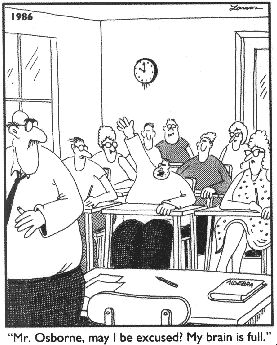
\includegraphics[scale=0.5]{brainisfull.jpg}
\end{center}
\end{frame}

\bfr{Learning requires a {\bf foundation of prior knowledge}}
\bi
\li {\bf Elaboration} is the practice of putting things in your own words
and connecting it to what you already know.\pause
\li If you practice elaboration there is no known limit to how
much you can learn.\pause
\bi
\li In 2010 Simon Reinhard memorized 300 random words in 15 minutes.
\li In 2008 Ben Pridmore memorized 884 shuffled playing cards in 30 minutes. 
\li In 2010 Boris-Nikolai Konrad memorized 201 names and faces in 15 minutes.
\ei\pause
\li All of these memory masters use mnemonic tricks that involve
relating the new knowledge to something they already know,
such as the ``memory palace.''
\ei
\end{frame}

\bfr{Learning changes your brain}
\bi
\li Many believe that their intellectual ability is hardwired at
birth.\pause
\li Every time you learn something you {\bf change your brain}.\pause
\li The hippocampus actually creates new neurons throughout your life.\pause
\li Understanding this enables you to see failure as a badge of
effort:  you need to dig deeper or try a different strategy.\pause
\li When learning is hard, you're doing important work.
\ei
\end{frame}

\bfr{The Testing Effect}
\bi
\li Tests: assessment {\em vs.} learning tool\pause
\li Aristotle:  {\em exercise in repeatedly recalling a thing
strengthens the memory}\pause
\li One experiment:
\bi
\li Subjects were given passages to read.
\li Some passages were immediately tested on.
\li Other passages were reread.\pause
\li {\bf Tested passages were remembered better.}
\ei
\pause
\li Another experiment:
\bi
\li Some subjects asked to memorize pairs like {\em foot-shoe}
\li Others asked to memorize pairs like {\em foot-s\_\_e}\pause
\li {\bf Second group did substantially better.}
\ei
\ei\pause
\centerline{\fbox{\sc Quizzing is a learning tool!}}
\end{frame}

\bfr{Spaced repetition}
\begin{center}
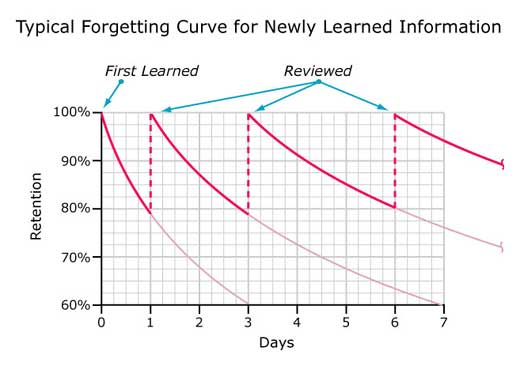
\includegraphics[scale=0.5]{ForgettingCurve.jpg}
\end{center}
\end{frame}

\bfr{Learning tips}
\bi
\li Practice retrieving from memory\pause
\bi
\li Use flash cards: \url{www.ankisrs.net}\pause
\li Use Cornell note taking system \\\url{http://lsc.cornell.edu/LSC_Resources/cornellsystem.pdf}\pause
\li Look up from the book and summarize\pause
\li Invent quiz questions as you read\pause
\li Don't listen to your intuition!
\ei
\ei
\end{frame}

\bfr{Learning tips}
\bi
\li Space out retrieval practice
\bi
\li No cramming
\li Use flash cards: {\tt www.ankisrs.net}
\li Avoid massed practice
\ei
\ei
\end{frame}

\bfr{Learning tips}
\bi
\li Interleave different study problems
\bi
\li Move back and forth in the text
\li Move between subjects
\li Move between study strategies
\ei
\ei
\end{frame}

\bfr{Learning tips}
\bi
\li Elaboration
\bi\li explain it in your own words and relate it to your own experience\ei
\ei
\end{frame}

\bfr{Learning tips}
\bi
\li Generation
\bi\li Try to answer a problem before being shown the solution\ei
\ei
\end{frame}

\bfr{Learning tips}
\bi
\li Reflection
\bi\li Write out essays on your learning\ei
\ei
\end{frame}

\bfr{Learning tips}
\bi
\li Calibration
\bi\li Use an objective instrument to assess yourself \ei
\ei
\end{frame}

\bfr{Learning tips}
\bi
\li Mnemonic devices
\bi
\li Mind maps
\li Memory palace
\li Think in vivid, crazy images
\li Major memory system for numbers
\ei
\ei
\end{frame}



\bfr{Learning tips}
\bi
\li Practice retrieving from memory
\li Space out retrieval practice
\li Interleave different study problems
\li Elaboration
\li Generation
\li Reflection
\li Calibration
\li Mnemonic devices
\ei
\end{frame}



\end{document}
